\chapter{Preliminaries of Differential Geometry}
\label{chap:diff_geom}

In this chapter we briefly introduce the foundations needed to understand the concept of supermanifolds and the Batalin-Vilkovisky formalism.
\textcolor{red}{Add more details of what it is said in the sections}.
We mostly refer to \cite{Nima} for this chapter on the basics of differential geometry.

\section{Vector Fields and Differential Forms}
\label{sec:sec1}

We start by defining the tangent space of a manifold at a particular point, given the definition of tangent vector.

\begin{definition}
    The \emph{tangent space} of a manifold $M$ at $q \in M$ is defined by the set of all tangent vectors at $q$.
\end{definition}

It is possible to map the tangent space $T_q M$ at $q \in M$ to a real vector space $\mathbb{R}^n$ through a bijection.
This bijection can be used to transfer the vector space operations of $\mathbb{R}^n$ to $T_q M$, thus turning the latter into a real vector space of dimension $n$.

The tangent space $T_q M$ of a manifold $M$ at point $q \in M$ is also used to define the dimension of the manifold 
\begin{equation*}
    \dim M \coloneqq \dim T_q M .
\end{equation*}

If we assemble together all the tangent vectors at all points $q$ of a manifold, we obtain the tangent bundle.

\begin{definition}
    The \emph{tangent bundle} of a manifold $M$ is given by the disjoint union of all tangent spaces on a manifold, thus
    \begin{equation*}
        TM \coloneqq \bigsqcup _{q \in M} T_q M .
    \end{equation*}
\end{definition}

An element of $TM$ is a pair $(q, v)$, where $q \in M$ and $v \in T_q M$.
There is a natural projection
\begin{align*}
    \pi : TM &\rightarrow M \\
    (q, v) &\mapsto q .
\end{align*}

More generally we can define a vector bundle over a manifold.
\begin{definition}
    A \emph{vector bundle} of rank $r$ is a triple $(E, \pi, M)$, where $E$ is an $r$-dimensional manifold called the \emph{total space}, $M$ is a manifold called the \emph{base space} and $\pi : E \rightarrow M$ is a continuous surjective map.
\end{definition}

We call the $r$-dimensional vector space $E_q \coloneqq \pi^{-1}(q)$ the \emph{fiber} at $q \in M$.
The tangent space is already an example of tangent bundle.

\begin{example}
    The Möbius strip is a vector bundle of rank $1$ over the circle $S^1$ (see \Cref{fig:Mobius}). Note that the product manifold $[-1, 1] \times S^1$ would be a cylinder, not the Möbius strip.
\end{example}

\begin{figure}
    \centering
    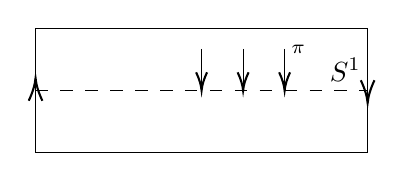
\begin{tikzpicture}[x=0.75pt,y=0.75pt,yscale=-1,xscale=1]
    %uncomment if require: \path (0,300); %set diagram left start at 0, and has height of 300
    
    %Straight Lines [id:da575614681710741] 
    \draw    (150,90) -- (310,90) ;
    %Straight Lines [id:da7355250432830472] 
    \draw    (150,150) -- (310,150) ;
    %Straight Lines [id:da425921249207598] 
    \draw  [dash pattern={on 4.5pt off 4.5pt}]  (150,120) -- (310,120) ;
    %Straight Lines [id:da15541437714065776] 
    \draw    (150,150) -- (150,90) ;
    \draw [shift={(150,114)}, rotate = 90] [color={rgb, 255:red, 0; green, 0; blue, 0 }  ][line width=0.75]    (10.93,-3.29) .. controls (6.95,-1.4) and (3.31,-0.3) .. (0,0) .. controls (3.31,0.3) and (6.95,1.4) .. (10.93,3.29)   ;
    %Straight Lines [id:da40082781733479333] 
    \draw    (310,90) -- (310,150) ;
    \draw [shift={(310,126)}, rotate = 270] [color={rgb, 255:red, 0; green, 0; blue, 0 }  ][line width=0.75]    (10.93,-3.29) .. controls (6.95,-1.4) and (3.31,-0.3) .. (0,0) .. controls (3.31,0.3) and (6.95,1.4) .. (10.93,3.29)   ;
    %Straight Lines [id:da6754846896588976] 
    \draw    (270,100) -- (270,118) ;
    \draw [shift={(270,120)}, rotate = 270] [color={rgb, 255:red, 0; green, 0; blue, 0 }  ][line width=0.75]    (8.74,-2.63) .. controls (5.56,-1.12) and (2.65,-0.24) .. (0,0) .. controls (2.65,0.24) and (5.56,1.12) .. (8.74,2.63)   ;
    %Straight Lines [id:da23038618406097078] 
    \draw    (250,100) -- (250,118) ;
    \draw [shift={(250,120)}, rotate = 270] [color={rgb, 255:red, 0; green, 0; blue, 0 }  ][line width=0.75]    (8.74,-2.63) .. controls (5.56,-1.12) and (2.65,-0.24) .. (0,0) .. controls (2.65,0.24) and (5.56,1.12) .. (8.74,2.63)   ;
    %Straight Lines [id:da41624213159172174] 
    \draw    (230,100) -- (230,118) ;
    \draw [shift={(230,120)}, rotate = 270] [color={rgb, 255:red, 0; green, 0; blue, 0 }  ][line width=0.75]    (8.74,-2.63) .. controls (5.56,-1.12) and (2.65,-0.24) .. (0,0) .. controls (2.65,0.24) and (5.56,1.12) .. (8.74,2.63)   ;
    
    % Text Node
    \draw (272,100) node [anchor=west] [inner sep=0.75pt]  [font=\scriptsize] [align=left] {$\displaystyle \pi $};
    % Text Node
    \draw (308,117) node [anchor=south east] [inner sep=0.75pt]   [align=left] {$\displaystyle S^{1}$};
    
    
\end{tikzpicture}
    \caption{Construction of the Möbius strip.}
    \label{fig:Mobius}
\end{figure}

We introduce now the definition of a section, which will be essential to define vector fields and differential $1$-forms.

\begin{definition}
    Let $(E, \pi, M)$ be a vector bundle. A \emph{section} on an open subset $U \subset M$ is a continuous map $\sigma : U \rightarrow E$ such that $\pi \circ \sigma = \text{id}_U$.
\end{definition}

We will denote the space of sections of a vector bundle $(E, \pi, M)$ by $\Gamma(E)$.

\begin{definition}
    A section $X \in \Gamma(TM)$ of the tangent bundle of a manifold $M$ is called a \emph{vector field}.
\end{definition}

A vector field is nothing else than a choice of a tangent vector at a point $q$ for all points $q \in M$.
We will denote the space of vector fields on a manifold $M$ by $\mathfrak{X}(M) \coloneqq \Gamma(TM)$.
In local coordinates ($x^i$) on $M$, we can write a vector field $X \in \mathfrak{X}(M)$ as

\begin{equation*}
    X = \sum_{i=1}^n X^i \frac{\partial}{\partial x^i}.
\end{equation*}

In particular, if $M = \mathbb{R}^n$, $X$ a smooth vector field and $f$ a smooth map, then we can define

\begin{equation*}
    X(f) = \sum_{i=1}^n X^i \frac{\partial f}{\partial x^i} .
\end{equation*}

\begin{definition}
    The \emph{cotangent bundle} $T^*M$ of a manifold $M$ is the dual of the tangent bundle $TM$.
\end{definition}

Similarly to what we did to define vector spaces, we can now introduce the concept of differential $1$-forms.

\begin{definition}
    A section $\omega \in \Gamma(T^*M)$ of the cotangent bundle of a manifold $M$ is called a \emph{differential $1$-form}.
\end{definition}

We denote by $\Omega^1(M) \coloneqq \Gamma(T^*M)$ the space of differential $1$-forms.

We now introduce the notion of tensor bundle in order to generalize vector fields and differential $1$-forms to multivector fields and differential $s$-forms, respectively.
We will then define the de Rham differential on $s$-forms, the Lie derivative and the contraction of a vector field with an $s$-form.

\begin{definition}
    Assume $(E, \pi, M)$ is a vector bundle over $M$.
    We define the \emph{tensor bundle} $T_s ^k (E)$ to be the vector bundle whose fiber at $q$ is the tensor bundle $T_s ^k (E_q) \coloneqq E_q ^{\otimes k} \otimes (E_q ^*) ^{\otimes s}$, where $\cdot^{\otimes k}$ denotes the $k$-th tensor power.
\end{definition}

When the total space $E$ of the vector bundle is the tangent bundle $TM$ of the manifold $M$, we can recover the definitions of multivector field and differential $s$-forms.
For this we need the \emph{alternating tensor product} $\wedge$, also called \emph{wedge product}.
We denote by $\text{Alt}_s ^k$ the tensor bundle induced by the wedge product $\wedge$ instead of by the tensor product $\otimes$.

\begin{definition}
    A \emph{multivector field $X$ of order $k$} is a section of the contravariant tensor field $\text{Alt}_0 ^k$.
\end{definition}

We denote the space of multivector fields of order $k$ by
\begin{equation*}
    \mathfrak{X}^k(M) \coloneqq \Gamma(\text{Alt}_0 ^k) = \Gamma \left( \bigwedge ^k TM \right).
\end{equation*}

\begin{definition}
    A \emph{differential $s$-form} $\omega$ is a section of the covariant tensor field $\text{Alt}_s ^0$.
\end{definition}

Similarly, we denote the space of differential $s$-forms by

\begin{equation*}
    \Omega ^s(M) \coloneqq \Gamma (\text{Alt}_s ^0 ) = \Gamma \left( \bigwedge ^s T^*M \right).
\end{equation*}

Choosing local coordinates ($x^i$) on $M$ we can represent the elements $X \in \mathfrak{X}^k(M)$ and $\omega \in \Omega^s(M)$ respectively as

\begin{align*}
    X &= \sum_{1 \leq i_1 < \ldots < i_k \leq n} X^{i_1 \ldots i_k} \partial_{i_1} \wedge \ldots \wedge \partial_{i_k} \\
    \omega &= \sum_{1 \leq i_1 < \ldots < i_s \leq n} \omega_{i_1 \ldots i_s} \dd x^{i_1} \wedge \ldots \wedge \dd x^{i_s}.
\end{align*}

\begin{definition}
    The \emph{contraction}, also called \emph{internal multiplication}, of a vector field $X$ with a differential $s$-form $\omega$ is defined as
    \begin{equation*}
        \iota_X \omega =
        \sum_{1\leq i_1 < \ldots < i_s \leq n} \sum_{k=1}^n (-1)^k
        \omega_{i_1 \ldots i_s} X^{i_k}
        \dd x^{i_1} \wedge \ldots \wedge \widehat{\dd x^{i_k}} \wedge \ldots \wedge \dd x^{i_s}
        \in \Omega^{s-1}(M),
    \end{equation*}
    where $\; \widehat{\cdot} \;$ means that the element is omitted.
\end{definition}

The definition of flow of a vector field is also needed in order to introduce the concept of Lie derivative.

\begin{definition}
    Let $M$ be a manifold and let $X$ be a vector field.
    Then the \emph{flow} of $X$ is the unique solution to the Cauchy problem
    \begin{align*}
        \pderivative{t} \Phi _t ^X (q) &= X(\Phi_t ^X (q)), \\
        \Phi_0 ^X (q) &= q,
    \end{align*}
    where $q \in M$ and $t$ is in the neighbourhood of $0$.
\end{definition}

\begin{definition}
    The \emph{Lie derivative} of an $s$-form $\omega$ with respect to a vector field $X$ is given by
    \begin{equation*}
        L_X \omega \coloneqq \lim _{t \rightarrow 0} \frac{(\Phi_t ^X)^* \omega - \omega}{t},
    \end{equation*}
    where $\Phi_t ^X$ is the flow of $X$ at time $t$.
\end{definition}

Thus, the Lie derivative $L_X \omega$ is the rate of change of $\omega$ in the direction of the flow of $X$.
\section{De Rham Cohomology}
\label{sec:derham}

In this section we introduce the notion of de Rham differential, followed by the concepts of a chain complex and in particular of de Rham cohomology.

\begin{definition}
    The \emph{de Rham differential} is defined as the map
    \begin{align*}
        \dd : C^{\infty}(M) &\rightarrow \Omega^1(M) \\
        f &\mapsto \dd f ,
    \end{align*}
    which is $\mathbb{R}$-linear and such that the Leibniz rule holds
    \begin{equation*}
        \dd (fg) = \dd fg + f \dd g, \quad \forall f, g \in C^{\infty}(M).
    \end{equation*}
\end{definition}

The de Rham differential can be quickly generalized to $s$-forms as
\begin{align*}
    \dd : \Omega^s (M) &\rightarrow \Omega^{s+1}(M) \\
    \omega &\mapsto \dd \omega .
\end{align*}

Explicitly, for an $s$-form $\omega = \sum_{1 \leq i_1 < \ldots < i_s \leq n} \omega_{i_1 \ldots i_s} \dd x^{i_1} \wedge \ldots \wedge \dd x^{i_s}$, we get

\begin{equation*}
    \dd \omega = \sum_{1 \leq i_1 < \ldots < i_s \leq n} \sum_{j = 1}^n \partial_j \omega_{i_1 \ldots i_s} \dd x^j \wedge \dd x^{i_1} \wedge \ldots \wedge \dd x^{i_s} .
\end{equation*}

It is easy to see that $\dd ^2 \omega = 0$, which will be an important fact in order to define the de Rham Cohomology group.
Here we quicly prove that $\dd^2 \omega = 0$, using the fact that partial derivatives commute while the wedge product anti-commute.
The second de Rham derivative of $\omega$ can be written as

\begin{equation*}
    \dd ^2 \omega =
    \sum_{1 \leq i_1 < \ldots < i_s \leq n} \sum_{j = 1}^n \sum_{k = 1}^n
    \partial_k \partial_j \omega_{i_1 \ldots i_s}
    \dd x^k \wedge \dd x^j \wedge \dd x^{i_1} \wedge \ldots \wedge \dd x^{i_s}.
\end{equation*}

For a particular $j=j'$ and $k=k'$, the element of the sum is

\begin{align*}
     \sum_{1 \leq i_1 < \ldots < i_s \leq n}
     &\partial_{k'} \partial_{j'} \omega_{i_1 \ldots i_s}
     \dd x^{k'} \wedge \dd x^{j'} \wedge \dd x^{i_1} \wedge \ldots \wedge \dd x^{i_s} = \\
     \sum_{1 \leq i_1 < \ldots < i_s \leq n}
     - &\partial_{j'} \partial_{k'} \omega_{i_1 \ldots i_s}
     \dd x^{j'} \wedge \dd x^{k'} \wedge \dd x^{i_1} \wedge \ldots \wedge \dd x^{i_s}
\end{align*}

which cancels with the term having $j = k'$ and $k=j'$.

Let us now introduce the notion of chain complexes.

\begin{definition}
\label{def:chain}
    Let $k$ be a ring. A \emph{chain complex} of $k$-modules is a sequence
    \begin{equation*}
        \begin{tikzcd}
            \ldots \rightarrow  C_{n+1} \arrow[r, "\dd _{n+1}"] & C_n
            \arrow[r, "\dd _{n}"] & C_{n-1} \rightarrow \ldots
        \end{tikzcd}
    \end{equation*}
    where $C_n$ denotes a $k$-module and $\dd _n$ is an homomorphism between $C_n$ and $C_{n-1}$ satisfying $\dd _n \circ \dd _{n-1} = 0$ for all $n \in \mathbb{Z}$.
\end{definition}

A chain complex as in \Cref{def:chain} is often denoted with $(C_{\bullet}, \dd)$ or just with $C_{\bullet}$.
In other words, a chain complex is a sequence of modules and a sequence of homomorphisms between consecutive modules such that the image of each homomorphism is included in the kernel of the next one.

If we now want to map to chain complexes to one another, we need to introduce the concept on chain map, which will be necessary to study the gluing properties of the space of fields on two manifolds.

\begin{definition}
\label{def:chain_map}
    A \emph{chain map} between two chain complexes $(C_\bullet, \dd \,)$ and $(\widetilde{C}_\bullet, \widetilde{\dd} \,)$ is denoted by $f_\bullet : C_\bullet \rightarrow \widetilde{C}_\bullet$ and is given by a collection of maps $f_n : C_n \rightarrow \widetilde{C}_n$ such that
    $f_n \circ \dd_{n+1} = \widetilde{\dd}_{n+1} \circ f_{n+1}$ for all $n \in \mathbb{Z}$.
    In other words, the maps $f_n$ have to satisfy the following commutative diagram
    \begin{equation*}
        \begin{tikzcd}
    \ldots \arrow[r, "\dd_{n+2}"] &
    C_{n+1} \arrow[r, "\dd_{n+1}"] \arrow[d, "f_{n+1}"] &
    C_{n} \arrow[r, "\dd_{n}"] \arrow[d, "f_{n}"] &
    C_{n-1} \arrow[r, "\dd_{n-1}"] \arrow[d, "f_{n-1}"] & \ldots \\
    \ldots \arrow[r, "\widetilde{\dd}_{n+2}"] &
    \widetilde{C}_{n+1} \arrow[r, "\widetilde{\dd}_{n+1}"] &
    \widetilde{C}_{n} \arrow[r, "\widetilde{\dd}_{n}"] &
    \widetilde{C}_{n-1} \arrow[r, "\widetilde{\dd}_{n-1}"] & \ldots
\end{tikzcd}
    \end{equation*}
\end{definition}

The requirement in \Cref{def:chain} of inclusion of the image of each homomorphism in the kernel of the next one allows us to introduce the concept of homology, which indeed describes how this inclusion takes place.

\begin{definition}
\label{def:homology}
    Let $(C_{\bullet}, \dd )$ be a chain complex.
    The \emph{$n$-th homology group} of $C_{\bullet}$ is defined as
    \begin{equation*}
        H_n (C_\bullet) \coloneqq \frac{\ker (\dd_n)}{\text{Im} (\dd_{n+1})}.
    \end{equation*}
\end{definition}

What we get by reversing the direction of the arrows in \Cref{def:chain} is known as \emph{cochain complex} and it is denoted by $C^\bullet$.
The homology of a cochain complex is called \emph{cohomology} and can simply be written as $H^n (C^\bullet) = {\ker (\dd_n)} / {\text{Im} (\dd_{n-1})}$.

In the particular case where the $k$-modules of the chain complex are the spaces of differential forms on an $n$-dimensional manifold $M$ and the homomorphisms between them are the de Rham differential, then we get what is called \emph{de Rham complex}:

\begin{equation*}
    0 \rightarrow C^\infty(M) \xrightarrow{\dd} \Omega^1(M)
    \xrightarrow{\dd} \ldots \xrightarrow{\dd} \Omega^s(M)
    \xrightarrow{\dd} \Omega^{s+1}(M) \xrightarrow{\dd} \ldots 
    \xrightarrow{\dd} \Omega^n(M)\rightarrow 0 .
\end{equation*}

Notice that the requirement $\! \dd^{(s-1)} \circ \dd^{(s)} = 0$ is satisfied by how the differential is constructed.
Similarly to \Cref{def:homology}, we can define the cohomology group of the de Rham complex.

\begin{definition}
    The \emph{$s$-th de Rham cohomology} of a de Rham complex of a manifold $M$ is given by
    \begin{equation*}
        H^s(M) \coloneqq \frac{\ker \Big( \dd : \Omega^s(M) \rightarrow \Omega^{s+1}(M)  \Big)}
        {\text{Im}\Big( \dd : \Omega^{s-1}(M) \rightarrow \Omega^{s}(M)  \Big)} .
    \end{equation*}
\end{definition}

In particular, we call the elements of $\ker \dd ^{(s)} \coloneqq \{ \omega \in \Omega^s(M) \, | \, \dd ^{(s)} \omega = 0\}$ \emph{closed forms} and the elements of $\text{Im} \, \dd ^{(s)} \coloneqq \{ \omega \in \Omega^s(M) \, | \, \exists \eta \in \Omega^{s-1}(M), \, \omega = \dd \eta \}$ \emph{exact forms}.
The property $\dd \circ \dd = 0$ tells us that all exact forms are also closed forms, since if $\omega \in \Omega^s(M)$ is exact then $\dd \omega = \dd ^2 \eta = 0$.
We will denote the collection of all de Rham cohomology groups as $H^\bullet(M)$.

\section{Symplectic Geometry}
\label{sec:symplectic_geom}

In this section we briefly introduce the concepts of symplectic forms on manifolds, Hamiltonian and symplectic vector fields.

Let $\omega$ be a $2$-form on a manifold $M$. Note that the map
\begin{equation*}
    \omega_q : T_q M \wedge T_q M \rightarrow \mathbb{R}
\end{equation*}
is skew-symmetric, meaning that
\begin{equation*}
    \omega(v, w) = -\omega(w, v), \quad \forall v, w \in T_q M.
\end{equation*}

If $\omega$ is skew-symmetric and non-degenerate, then is called a \emph{symplectic form}.

\begin{definition}
    A 2-form $\omega \in \Omega^2(M)$ is called \emph{symplectic} if $\omega$ is closed and $\omega_q$ is symplectic for all $q \in M$.
\end{definition}

It directly follows the definition of symplectic manifold.
\begin{definition}
\label{def:sympl_mnf}
    A pair $(M, \omega)$, where $M$ is a manifold and $\omega$ is a symplectic form, is called a \emph{symplectic manifold}.
\end{definition}

Recall now that the contraction with a vector field $X \in \mathfrak{X}(M)$ of a $2$-form is a map

\begin{equation*}
    \iota_X : \Omega^2(M) \rightarrow \Omega^1(M).
\end{equation*}

If we let $M$ be a symplectic manifold with a symplectic form $\omega$, then by non-degeneracy of $\omega$ it is possible to find a unique vector field $X_H$ such that its contraction with $\omega$ is equal to the de Rham differential of a particular smooth function $H \in C^\infty(M)$, called Hamiltonian function.

\begin{definition}
    Let $(M, \omega)$ be a symplectic manifold and $H:M\rightarrow \mathbb{R}$ a smooth function.
    A vector field $X_H \in \mathfrak{X}(M)$ satisfying
    \begin{equation*}
        \iota_{X_H}\omega = \dd H
    \end{equation*}
    is called \emph{Hamiltonian vector field} with \emph{Hamiltonian function} $H$.
\end{definition}

In particular, since the $1$-form $\iota_{X_H} \omega$ is the de Rham differential of a function $H$, this means that $\iota_{X_H} \omega$ is exact.
On the other hand, if $\iota_X \omega$ is closed, using Cartan's magic formula, we can compute the Lie derivative

\begin{equation*}
    L_X \omega = \iota_X \dd \omega + \dd \iota_X \omega = 0,
\end{equation*}
since $\omega$ is closed for being a symplectic form.

\begin{definition}
    A vector field $X$ on a symplectic manifold $(M, \omega)$ such that $L_X \omega = 0$ is called \emph{symplectic vector field}.
\end{definition}

Since, by definition, a symplectic manifold is endowed with a symplectic form $\omega$, it is then possible to define the Poisson bracket on the manifold.
\begin{definition}
    The \emph{Poisson bracket} of two functions $f, g \in C^\infty(M)$ on a symplectic manifold $(M, \omega)$ is defined by
    \begin{equation*}
        \{f, g\} \coloneqq \omega(X_f, X_g) .
    \end{equation*}
\end{definition}
In the definition above, the notation $X_f$ denotes the vector field associated with $f$ such that $\iota_{X_f} \omega = \dd f$ holds.
Thus, it is the Hamiltonian vector field associated to the Hamiltonian function $f$ (the same applies for the function $g$).
